\begin{exercise}{Pendule simple incliné}{2}{Sup}
{Mécanique, Moment cinétique}{correge}

On réalise un pendule simple à l’aide d’un mobile autoporteur sur table à coussin d’air. Le mobile de masse $m$ est accroché à l’extrémité d’un fil de longueur $\ell$ dont l’autre extrémité est attachée à un point fixe $O$ de la table.Le mobile peut alors se déplacer sans frottement dans un plan $xOy$.

\begin{center}
    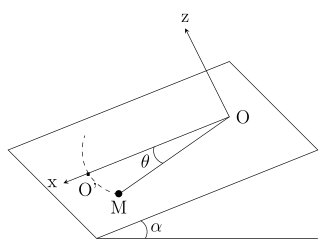
\includegraphics[scale=0.6]{meca/mecasolides/pendule_incline}
\end{center}

\begin{questions}
    \questioncours Moment cinétique.
    \question Exprimer le moment cinétique de $M$ par rapport à $O$.
    \question Identifier les forces et exprimer leur projection sur la base cylindrique.
    \question Appliquer le théorème du moment cinétique afin d’établir l’équation différentielle du mouvement dans le cas des petites oscillations.
    \question En déduire l’expression de la période des petites oscillations.
    \question Le pendule est lancé depuis sa position d’équilibre $O$’ avec un vitesse initiale $v_0$. Quel est l’angle maximal atteint (l’hypothèse des petites oscillations étant toujours valable) ?
\end{questions}

\end{exercise}

\begin{solution}
\begin{questions}
    \questioncours 
    \question $L = m\ell^2 \dot{\theta}^2$
    \question $\vec{P} = mg(\sin \alpha \cos \theta, -\sin \alpha \sin \theta,  -\cos \alpha)_{(r,\theta,z)}$
    \question $\ddot \theta + \theta \frac{g}{\ell}\sin \alpha = 0$
    \question $\omega_0^2 = \frac{g}{\ell}\sin \alpha$
    \question On trouve la solution, et on cherche le maximum. On trouve $\theta_{max} = \frac{v_0}{\ell \omega_0}$
\end{questions}

\end{solution}

